%
% Bachelorarbeit
% Phil Diegmann
%

% -----------
% 1. Präambel
% -----------

% Allgemeine Einstellungen
% ------------------------
\documentclass[
    pdftex,
	a4paper,
	oneside,
	12pt,
	liststotocnumbered
]{article}

\usepackage{times}            % Times New Roman
\usepackage{newclude}
\usepackage[ampersand]{easylist}

\usepackage[utf8]{inputenc}   % utf-8
\usepackage[T1]{fontenc}      % Umlauttrennung
\usepackage[english]{babel}    % englische Silbentrennung
\selectlanguage{english}       % englische Betitelung
\usepackage{nicefrac}

% Titel-Font-Größen
\usepackage{titlesec}
\titleformat{\section}{\bfseries}{\thesection.}{12pt}{}
\titleformat{\subsection}{\bfseries}{\thesubsection }{12pt}{}

% Seitenränder
\usepackage[
    top=2.5cm, 
    bottom=2.5cm, 
    left=5cm, 
    right=1cm
]{geometry} 

% Fussnoten
\usepackage[hang,flushmargin]{footmisc}    
\renewcommand*{\footnotelayout}{\footnotesize} % size of text
\renewcommand{\footnotemargin}{2.2em}          % margin between text and number
\setlength{\footnotesep}{1.3em}                % space between footnotes
\setlength{\skip\footins}{2.5em}               % space between text & footnotes
\usepackage{savefnmark}

% Abkürzungen
%[printonlyused]
\usepackage{acronym}
\renewcommand{\bflabel}[1]{{#1\hfill}}

% Seitennummerierung oben
\usepackage{scrpage2} 
\usepackage[dvips]{color}
\clearscrheadfoot 
\chead[\pagemark]{\textcolor[gray]{0.5}{\pagemark}} 
\pagestyle{scrheadings}

% TOC, LOF, FIG Styles
\usepackage{needspace}
\usepackage{tocloft, titletoc}  
\setlength{\cftaftertoctitleskip}{0em}
\usepackage[colorlinks=false]{hyperref}
\renewcommand{\cftloftitlefont}{\bfseries}
%\renewcommand{\cftfigfont}{\bfseries}
\renewcommand{\cfttoctitlefont}{\bfseries}
\renewcommand{\cftlottitlefont}{\bfseries}
\titlecontents{section}     % set formatting for \section 
[2.3em]                     % adjust left margin
{\vspace{0.5em}}            % font formatting
{\hspace{-1.8em}.\contentslabel{0.7em}\hspace{1em}} % section label and offset
{\hspace*{-2.3em}}
{\titlerule*[1mm]{.}\contentspage}

\titlecontents{subsection}  % set formatting for \subsection 
[3em]                       % adjust left margin
{\vspace{0.5em}}            % font formatting
{\contentslabel{2.3em}}     % section label and offset
{\hspace*{-2.3em}}
{\titlerule*[1mm]{.}\contentspage}

\titlecontents{subsubsection}  % set formatting for \subsubsection 
[4.2em]                       % adjust left margin
{\vspace{0.5em}}            % font formatting
{\contentslabel{2.3em}}     % section label and offset
{\hspace*{-2.3em}}
{\titlerule*[1mm]{.}\contentspage}

\titlecontents{figure}      % set formatting for \subsection 
[2.3em]                     % adjust left margin
{\vspace{0.5em}}            % font formatting
{\contentslabel{2.3em}}     % section label and offset
{\hspace*{-2.3em}}
{\titlerule*[1mm]{.}\contentspage}

\titlecontents{table}       % set formatting for \subsection 
[3.4em]                     % adjust left margin
{\vspace{0.5em}}            % font formatting
{:\hspace*{0.9em}\contentslabel{4.5em}}     % section label and offset
{\hspace*{-2.3em}}
{\titlerule*[1mm]{.}\contentspage}


% Literaturverzeichnis
\usepackage[
    bibstyle=authortitle,
    citestyle=authoryear,
    isbn=false,
    url=false,
    doi=false,
    maxcitenames=3,
    maxbibnames=30
]{biblatex}
\addbibresource{literature.bib}
\let\cite\textcite

\usepackage{caption}
\usepackage{chngcntr}

% Tabellenpackete
\usepackage{array}
\usepackage{xcolor}
\usepackage{longtable}
\usepackage{setspace}
\counterwithin{table}{section}
\usepackage{multirow}
\usepackage{longtable}

% Grafiken anzeigen
\usepackage[pdftex]{graphicx}
\graphicspath{{figures}}
\counterwithin{figure}{section}
\usepackage[absolute,overlay]{textpos}

\setlength{\parindent}{0in}

\begin{document}
%\shorthandoff{"}

% Renews
\renewcommand{\figurename}{Abb.}
\renewcommand{\tablename}{}
\renewcommand\thefigure{\arabic{section}-\arabic{figure}}
\renewcommand\thetable{Tab. \arabic{section}-\arabic{table}}
\newcommand{\todo}[1]{\textbf{\textsc{\textcolor{red}{TODO: #1}}}}
\renewcommand{\contentsname}{Table of Contents}

\pagenumbering{Roman}

% ---------
% Deckblatt
% ---------
\vspace*{1mm}

% Name
\thispagestyle{empty}
Phil Diegmann

\vspace*{23mm}

% Bacheloararbeit
\begin{center}
\textbf{
    Bachelorarbeit
\linebreak
    im Fach Allgemeine Wirtschaftsinformatik}
\end{center}

\vspace*{20mm}

% Titel
\begin{center}
\LARGE 
    Development of mHealth Apps – Discovering the Dos and Don'ts in the Case of ePill
\end{center}

\vspace*{8mm}

% Themensteller
\begin{center}
    Themensteller: Jun.-Prof. Dr. Ali Sunyaev
\end{center}

\vspace*{12mm}

% Vorgelegt
\begin{center}
    Vorgelegt in der Bachelorprüfung
\linebreak
    im Studiengang Wirtschaftsinformatik
\linebreak
    der Wirtschafts- und Sozialwissenschaftlichen Fakultät
\linebreak
    der Universität zu Köln
\end{center}

\vspace*{30mm}

% Köln, September 2013
\begin{center}
Köln, September 2013
\end{center}





% ------------------
% Inhaltsverzeichnis
% ------------------
\tocloftpagestyle{scrheadings}
\tableofcontents
\newpage

% ---------------------
% Abkürzungsverzeichnis
% ---------------------
\section*{Index of Abbreviations}
\addcontentsline{toc}{section}{Index of Abbreviations}
\begin{longtable}{@{}p{.275\textwidth}@{}p{.725\textwidth}@{}}
    app & Application \\
    app user & intended audience for the app \\
    CDN & Content Delivery Network. Multiple servers which are globally distributed for serving static content with high availability and performance \\
    CSS & Cascading Style Sheets. A language used to style web pages \\
    DNS & Domain Name System. Used to translate domain names into IP-Addresses \\
    eHealth & "a paradigm involving the concepts of health, technology, and commerce, with commerce and technology as tools in the service of health"\footnote{\cite{MartinezPerez.2013}, p. 2}. eHealth belongs to the field of telehealth.\footnote{cf. \cite{MartinezPerez.2013}, p. 2} \\
    ePill & a patient-centered health IT service which offers information on pharmaceuticals and aggregation of data in context\footnote{cf. \cite{Dehling.2012b}, p. 2} \\
    framework & can contain source code, tools and libraries, which together provide specific or common but abstracted functionality \\
    frontend & visible user interface for the app user \\
    HECAT & Health Education Curriculum Analysis Tool\footnote{\url{http://www.cdc.gov/HealthyYouth/HECAT/}} \\
    HIT & abbreviation for Health Information Technology \\
    HTML & HyperText Markup Language, a markup language to design web pages \\
    IDE & Integrated Development Environment \\
    JSON & JavaScript Object Notation, represents data structures \\
    mHealth & "medical and public health practice supported by mobile devices, such as mobile phones, patient monitoring devices, personal digital assistants (PDAs), and other wireless devices"\footnote{\cite{WorldHealthOrganization.2011} cited by \cite{MartinezPerez.2013}, p. 2}, also known as m-Health \\
    mHealth apps & "aim at providing seamless, global access to tailored health IT services and have the potential to alleviate global health burdens"\footnote{\cite{Dehling.2013}, p. 1} \\
    MVC & Model-View-Controller. A software architecture pattern which separates logic and user interfaces. Models are representatives of data structures. Views contains the user interface definitions and controllers contains the application logic \todo{cite} \\
    NDK & Native Development Kit. Bundled software and tools which enables the developer to implement programs on native-code languages\footnote{cf. \url{http://developer.android.com/tools/sdk/ndk/index.html}} \\
    OS & Operating System \\
    SDK & Software Development Kit. Bundled software and tools for developing with or for a specified OS or framework \\
    telehealth & delivery of medical- or health-related information or services via telecommunication technologies \\
    usability & "extent to which a product can be used by specified users to achieve specified goals with effectiveness, efficiency and satisfaction in a specified context of use"\footnote{\cite{Yeh.2012}, p. 64 as quoted from ISO 9241-11 (1998)} \\
    use value & the utility of consuming a good or service \\
    user interface & for humans visible controls and layout of an application \\
    W3C & World Wide Web Consortium\footnote{\url{http://www.w3.org}} \\
\end{longtable}

% -------------------
% Tabellenverzeichnis
% -------------------
%\listoftables
%\addcontentsline{toc}{section}{Index of Tables}
%\newpage

\normalsize
\setstretch{1,5}
\pagenumbering{arabic}

% ------
% Inhalt
% ---------
\section{Introduction}
\subsection{Research Problem}
While it has become easy to develop a mobile health (mHealth) application (app), there is much more to it than just the aspects of the app's core functionality. Currently only very few guidelines, best practices and systematic development approaches for mobile app development can be found. Furthermore even less can be found for the specific area of mHealth apps.
\\
\\
Security leaks or even abuse of private and sensitive information\footnote{information, which is personal. Can be related to financial-, health- or otherwise personal relevant information, suggested by \cite{FutureofPrivacyForumCenterforDemocracy&Technology.2011}, p. 6, although the definition varies} can lead to great harm for the app user and to legal issues for the developer. Abuse of personal health related information can result in loss of reputation (e.g. sexual transmitted diseases) or financial drawbacks and decreased chances of employment (e.g. chronic diseases, genetic dispositions)\footnote{cf. \cite{Dehling.2013}, pp. 6-7}. With poorly developed apps, there is a danger of security leaks and hence for data abuse. Thus the risk for app users increases. A study has shown that very few mHealth apps entail little or low risk for the app user.\footnote{cf. \cite{Njie.2013}, pp. 19-20} Self-publishing through modern sales channels such as Google Play\footnote{\url{http://play.google.com}} or the iOS App Store \footnote{\url{http://appstore.com}} and the availability of easy-to-use Integrated Development Environments (IDEs) lower the barriers for entry. Even one-man developers or small teams are now able to publish apps with less development effort than a few years ago.\footnote{cf. for this and the next sentence \cite{Dehling.2013}, p. 2}\footnote{cf. for this and the next sentence \cite{Moore.2012}, p. 15} Without fundamental knowledge of privacy and security aspects, there is an increase in the non-professional developmental of mobile apps with possibly inadequate security aspects.
\\
\\
Usability as well as the overall app quality is also a possibly undervalued aspect in non-professional developments.\footnote{cf. \cite{Dehling.2013}, p. 2}\footnote{cf. \cite{Mayer.2012}, p. 1681} While fancy colors might look appealing to the developer himself, it might lead to confusion for the app user or even to a lack of operability for visually impaired people.\footnote{cf. \cite{Badashian.2008} p. 108} Also, the need for a intuitive user interface\footnote{for humans visible controls and layout of an application} is not be considered as important as it should be.
\\
\\
Knowledge of data privacy acts and laws is a premise for a legal, safe and fair development for the developer and the app user. Multiple layers of data privacy laws in Europe on international, national and state level require a certain legal knowledge.\footnote{cf. Directive 95/46 of the European Parliament and of the Council (October, 24th 1995), Directive 2002/58 of the European Parliament and of the Council (July, 12th 2002) cited by \cite{FutureofPrivacyForumCenterforDemocracy&Technology.2011}, p. 16} Also, the benefit of and the need for a privacy policy seems to be ambiguous for many non-professional developers.\footnote{cf. \cite{Njie.2013}, p. 20}
\\
\\
This lack of guidelines for mobile app development and of specific guidelines for privacy and usability sensitive apps is only superficially considered by most of the literature. The beforehand highlighted aspects of usability and information security\footnote{information security stands for prevention from unauthorized access, modification, use or disruption of information and information systems} are just two of multiple possible requirements. Current research seems not to state which specific requirements, if any, distinguish mHealth apps from other apps or which are needed to be more accented.

\subsection{Objectives of this Thesis}
The purpose of this thesis is to discover, identify and report issues and challenges of the development of mHealth apps by developing a mobile frontend for the ePill system (developed by the University of Cologne, http://epill.uni-koeln.de). ePill is a patient-centered health IT service which offers information on pharmaceuticals and aggregation of pharmaceutical data in context.
\\
\\
During the development of a mobile frontend for ePill, all requirements can be addressed more easily than in a completely theoretical context. As a side effect, a mobile app for ePill will increase the accessibility for the ePill system in general, and thereby increase the possible user value. In critical situations in which one does not have a desktop computer at hand, a mobile easy-to-use app can be of value.
\\
\\
The experiences gained during the development refer to general mobile app development, but also to the specific development of mHealth apps.
\\
Mainly this thesis aims to describe the planning and the development process and discuss all discovered issues and challenges for planning and developing mHealth apps. One sub-objective is to give a short overview about the state of research on guidelines and important factors of mHealth app development. We will validate the developed app by reference to the stated guidelines and best practices. Also we aim to provide an short overview over different frameworks, compare them and give a short evaluation about the framework we chose for the implementation of the mobile frontend for ePill.
\newpage
\section{The ePill System}

\subsection{The System in general}
The ePill system (http://epill.uni-koeln.de) was developed by the University of Cologne to improve the readability and comprehensibility of instruction leaflets of medical drugs. Additionally ePill aims to provide further information on adverse reactions and interactions of different medical drugs. ePill emphasizes an easy readability and access to informations.
\\
There are three major functions covered by the system: Searching for pharmaceuticals, display information on pharmaceuticals and supplementing services.\footnote{cf. for this section \cite{Dehling.2012}, p. 2} The search enables the user to find corresponding pharmaceuticals depending on specified parameters in the underlying database. As an extend, the display functionality enables the user to read the leaflet information in an optimized fashion. Finally supplementing services are provided to refine the displayed information (e.g. select the level of detail of the displayed information), linking pharmaceuticals as well as other information and aggregate pharmaceutical information (e.g. interactions).
\\
An integration and personalization depending on the current user's health records was not implemented due to the arising privacy and trust challenges.\footnote{cf. \cite{Kaletsch.2011} cited by \cite{Dehling.2012}, p. 2}\footnote{cf. \cite{Kaletsch.2011}, pp. 5-6}

\subsection{The Web Application}
The web application of the ePill system introduces itself highly customizable to the user. Right 
\newpage
\section{What is mHealth?}

\subsection{Definition}
\todo{More Detail!}
\\
mHealth, also known as m-Health, is an abbreviation for mobile health and is a refinement of eHealth (or e-Health, an abbreviation for electronic health), which itself belongs to the field of telehealth.\footnote{cf. \cite{MartinezPerez.2013}, p. 2}
\\
\\
eHealth is defined as "a paradigm involving the concepts of health, technology, and commerce, with commerce and technology as tools in the service of health".\footnote{\cite{MartinezPerez.2013}, p. 2}
\\
\\
Telehealth means the delivery of medical- or health-related information or services via telecommunication technologies.
\\
\\
mHealth in detail is defined as "medical and public health practice supported by mobile devices, such as mobile phones, patient monitoring devices, personal digital assistants (PDAs), and other wireless devices".\footnote{\cite{WorldHealthOrganization.2011} cited by \cite{MartinezPerez.2013}, p. 2} The introduction of smart phones like the Apple iPhone or any Android device led to a greater audience and the evolution of mobile tablets further increased the audience for mHealth purposes. A study\footnote{cf. for this and the first following sentence \cite{West.2012}} relied on the Health Education Curriculum Analysis Tool (HECAT)\footnote{\url{http://www.cdc.gov/HealthyYouth/HECAT/}} to group different mHealth apps together. This study illustrates the distribution of apps in different categories. As \ref{tab:HECAT} illustrates, most of the available apps in 2011 in the Apple App Store in the United States of America belonged to the Physical Activity area, whereas drug-related and safety-related apps (like ePill) are the least two. 
\begin{table}[!htb]
    \center
    \begin{tabular}{l | c | c}
        \textbf{HECAT content area} & \textbf{n} & \textbf{\%}\footnotemark \\
        \hline
        Physical Activity & 1108 & 33.21 \\
        \hline
        Personal health and wellness & 962 & 28.84 \\
        \hline
        Healthy eating & 651 & 19.51 \\
        \hline
        Mental and emotional health & 414 & 12.41 \\
        \hline
        Sexual and reproductive health & 243 & 7.28 \\
        \hline
        Alcohol, tobacco, and other drugs & 131 & 3.93 \\
        \hline
        Violence prevention and safety & 96 & 2.88 \\
    \end{tabular}
    \caption[HECAT Content Area App Distribution]{HECAT Content Area App Distribution (N = 3336)\footnotemark}
    \label{tab:HECAT}
\end{table}
\addtocounter{footnote}{-1}
\footnotetext{Apps could be added to multiple categories}
\addtocounter{footnote}{1}
\footnotetext{cf. \cite{West.2012}, p. 5, Table 2}
\\
From February to May of 2012, a Study by \cite{dHeureuse.2012} found several ten thousands of apps in the Google Play Store as well as the Apple App Store just in the "Health" categories.\footnote{cf. \cite{dHeureuse.2012}, p. 20, Figure 5} This study shows the potential of mHealth for a broader healthcare supported by mobile devices. From March to May of 2012, the total number of apps increased by an average of 6.4\% (Google Play Store) and 4.5\% (Apple App Store) per month.\footnote{cf. \cite{dHeureuse.2012}, p. 20}

\subsection{mHealth App Categories}
Although the \ref{tab:HECAT} listed categories for mHealth apps, it focusses on content and less on the specifics for mHealth apps on other possibly important topics, such as information security or usability. Other literature focusses on data practices and privacy risks with a more technical aspect\footnote{cf. for this and the following three sentences \cite{Njie.2013}, pp. 13-14}. 
\\
\\
\cite{Njie.2013} concludes that most of the mHealth apps deal in any way with directly or indirectly (e.g. via usage behavior) with sensitive information. Therefor ten levels of privacy risks were developed and a sample of 43 mHealth and fitness apps were assigned to the different levels. \ref{tab:RiskLevelsmHealth} illustrates the characteristics of every level as well as the distribution of the 43 analyzed apps. 
\\
The risk levels are based on the one hand on the information available to the app and on the other hand security precautions implemented by the developer to prevent unauthorized access to this information. An important differentiation is also in the anonymity or identifiability of the information accessible by third parties. The higher the accessibility or the identifiability or the possible harm done by this information, the higher the risk level.
\\
\\
As stated by \cite{Istepanian.2004}, another categorization is possible. They categorized mHealth applications into administrative connectivity, financial connectivity or medical connectivity.\footnote{cf. \cite{Istepanian.2004}, p. 6} Because of the lack of smart phones and a far lesser availability of mobile devices in 2004 compared to today, this article cannot take the recent development in mobile devices into account. Nevertheless the categorization is still appropriate. The administrative connectivity handles appointments, electronic patient records and any non-financial transactions, the financial connectivity handles all financial transactions like purchases, billing or any financial services.\footnote{cf. for this and the first following sentence \cite{Istepanian.2004}, p. 13} The third connectivity, the medical connectivity, handles mobile monitoring and diagnostics.
\\
\begin{table}[!htb]
    \center
    \begin{tabular}{c | c | p{22.5em} | c}
        \textbf{Level} & \textbf{Risk} & \textbf{Characteristics} & \textbf{\%}\\
        \hline
        9 & Highest & address, financial information, full name, sensitive or embarrassing health (or health-related) information, information that a malicious actor could use to steal or otherwise cause a user to lose money & \multirow{3}[20]{*}{40} \\
        \cline{1-3}
        8 & High & geo-location & \\
        \cline{1-3}
        7 & Medium-high & DOB, ZIP code, any kind of personal medical
information & \\
        \hline
        6 & Medium & risk evaluated to be between level 5 and level 7 & \multirow{3}[12]{*}{32} \\
        \cline{1-3}
        5 & Medium & email, first name, friends, interests, weight, information that is potentially embarrassing or could be used against a person (e.g., in employment)\\
        \cline{1-3}
        4 & Medium & risk evaluated to be between level 5 and level 3\\
        \hline
        3 & Medium-low & anonymized (not personally identifiable) tracking (e.g., app usage), device info, a third party knows the user is using a mobile medical app & \multirow{3}[22]{*}{28} \\
        \cline{1-3}
        2 & Low & risk evaluated to be between level 3 and level 1\\
        \cline{1-3}
        1 & Low & any kind of anonymized data that does not include medical
health-related data or personally identifiable information\\
        \hline
        0 & No & & 0 \\
    \end{tabular}
    \caption[Privacy Risk Levels of mHealth Apps]{Privacy Risk Levels of mHealth Apps (N = 43)\footnotemark}
    \label{tab:RiskLevelsmHealth}
\end{table}
\footnotetext{cf. \cite{Njie.2013}, p. 13}
\\
There are there different sub-categories for mHealth applications: The content, the information security risk-level and the overall connectivity function. For the content-category as well as the connectivity-category, multiple assignments are possible. Combined these sub-categories form a specific grouping of mHealth apps. Depending on the categorization in the privacy risk, one can easily take care for precautions. With the categorization into a HECAT content area, one can identify the target audience more precisely as well as with the help of the connectivity category.

\subsection{Classification of the ePill Web Application}
ePill is to be categorized in the beforehand mentioned HECAT content areas mainly as "Alcohol, tobacco, and other drugs", because of the purpose to inform about (medical) drugs. Additionally, ePill informs about adverse effects and interactions, so it also belongs to the content area of "Violence prevention and safety".
\\
\\
The ePill web application is not connected to any electronic patient records, nor does it store any user related information, like the last searched pharmaceuticals. But it does not utilize SSL-encryption. Therefor it might not be collecting information or storing anything, but third parties could collect user specific information by monitoring.
\\
Setting this information into context with the risk levels developed by \cite{Njie.2013}, the ePill web application could be categorized as level three, if SSL-encryption would be utilized. If that would be the case, third parties could retrieve browser and OS specific information, but not data sent and retrieved with each request like pharmaceutical information. Without encryption, all data sent and retrieved is visible to possible eavesdropper. With information about searched pharmaceuticals, one could assemble a overall picture of the ingested drugs and therefor extrapolate possible diseases. Still, all data is anonymized.
\\
Having in mind, that ePill still is in early prototyping and assuming, that the SSL-encryption will follow, the risk is more of a medium to low level. Dealing with only anonymous data and protecting them with encryption leaves only very less room for serious risks. We would therefor categorize ePill in terms of privacy risk levels as a level two.
\\
\\
Although ePill does not fit absolutely in any of the connectivity categories, it fits best into the medical connectivity. Because of the aim to provide pharmaceutical (therefor medical) information, it belongs definitely to the medical connectivity category.
\\
\\
Concluding this categorization, we would suggest to categorize the ePill web application as a low privacy risk, drug- and safety-related medical connectivity mHealth application.
\\
The ePill web application lacks a optimization for mobile devices but all categorizations match their definition. The HECAT content area is by definition not limited to mobile devices and privacy risks are in many ways the same for mobile apps and web applications.

\subsection{Why is a special Focus on mHealth Apps warranted?}
mHealth apps differ in some way from general (mobile) applications but also from eHealth applications. While mHealth apps can be used in many different situations and with very different intentions, the special focus on e.g. equality of all users and accessibility for all possible users are not as important for other areas of mobile apps as they are for mHealth apps. 
\\
\\
mHealth apps are defined to "aim at providing seamless, global access to tailored health IT services and have the potential to alleviate global health burdens."\footnote{\cite{Dehling.2013}, p. 1}, which means, that they should be accessible by mostly all possible users, whereas other types of apps do not necessarily need to be accessible by any user. We want to stress, that accessibility does not only mean usability (especially for elderly people), but also e.g. different social layers or cultures.
\\
\\
Furthermore, mHealth apps deal with medical- or health-related information and have therefor to deal wit sensitive information and are to address privacy risks and concerns. As pointed out by \cite{Njie.2013} and already referred to in \ref{tab:RiskLevelsmHealth}, many mHealth apps deal with highly sensitive data and have serious privacy risks. \cite{Dehling.2013} illustrate the possible damages through leaks, manipulation or loss of information.\footnote{cf. \cite{Dehling.2013}, p. 7}
\\
\\
To address these concerns and issues in a mHealth project, they need to be made clear and experiences must be shared as well as interpreted. The following chapter will present all experiences made during the development of a mobile frontend for ePill in a structured way. We will list all theoretical preconditions, outline the analysis as well as the implementation of the mHealth app. Afterwards we will validate the product and give an overview about the lessons we learned.
\newpage
\section{The Development of the mobile Client}
\subsection{Preconditions}
\subsubsection{Norms for mobile Apps}
As already mentioned, ePill is currently only used in Germany, therefor we will focus on laws applicable in Germany. These laws are namely the \TKGns, the \TMGns, the \REG as well as the \DPA of \NRWns. The \TKG and \TMG are laws by state, whereas \REG is an european directive, specified by the respective Member States. 
\\
German federal states have their own \DPAsns. In this thesis we will focus on the \DPA of \NRW as ePill is located in \NRWns.
\\
\\
As the topmost layer of laws, the \REG defines more general directives. Article 4 defines national law applicable, if the natural or legal person, the controller\footnote{cf. \cite{TheEuropeanParliamentandtheCounciloftheEuropeanUnion.24.10.1995}, Article 2, (d)}, is located on a Member State's territory\footnote{cf. \cite{TheEuropeanParliamentandtheCounciloftheEuropeanUnion.24.10.1995}, Article 4, 1., (a) and (b)} or if any of the processing takes place on a Member State's territory\footnote{cf. \cite{TheEuropeanParliamentandtheCounciloftheEuropeanUnion.24.10.1995}, Article 4, 1., (c)}. Furthermore it is required, that the controller asks the user to consent to the use and collection of data\footnote{cf. \cite{TheEuropeanParliamentandtheCounciloftheEuropeanUnion.24.10.1995}, Article 7, (a)}, explicitly "data concerning health and sex life"\footnote{\cite{TheEuropeanParliamentandtheCounciloftheEuropeanUnion.24.10.1995}, Article 8, 1.} shall not be processed. Only if the user consents explicitly\footnote{cf. \cite{TheEuropeanParliamentandtheCounciloftheEuropeanUnion.24.10.1995}, Article 8, 2., (a)} or if the processing is done by a healthcare professional under national law and for preventive medicine, medical diagnosis or treatment or for the management of health-care services\footnote{cf. \cite{TheEuropeanParliamentandtheCounciloftheEuropeanUnion.24.10.1995}, Article 8, 3.}. 
\\
\\
This is refined by the the \TMGns. § 13, section (1) states, that the controller has to inform the user in a commonly understandable manner about the data which is collected and the form of processing of this data\footnote{cf. \cite{BundesregierungderBundesrepublikDeutschland.01.03.2007}, § 13, section (1)}. For a legal consent, the controller has to ensure, that the user is aware of his consent, that the consent is minuted, that the content of the consent is always available to the user and that the user can revoke his consent\footnote{cf. \cite{BundesregierungderBundesrepublikDeutschland.01.03.2007}, § 13, section (2)}.
\\
§§ 91, 93 and 94 of the \TKG states the same laws\footnote{cf. \cite{BundesregierungderBundesrepublikDeutschland.01.08.1996}, Section 2, §§ 91, 93, 94}.
\\
Also the \DPA of \NRW constitutes the same laws\footnote{cf. \cite{DerInnenministerdesLandesNordrheinWestfalen.09.06.2000}, Section 1, §§ 2, 4, 5} with the only restrictions, that its scope is limited to \NRWns.
\\
\\
Therefor ePill should explicitly inform the user that no data is stored and only anonymized transacted to find matching results, to comply with the stated laws.

\subsubsection{Best Practices}
The World Wide Web Consortium (W3C) has published a document in 2008 which states the basic best practices for developing for the mobile web. This document states 60 best practices, which shall ensure a minimum quality level for mobile web applications. These best practices emphasize the need of regard of the device's capabilities and supported technologies\footnote{cf. \cite{WorldWideWebConsortium.2008}, e.g. 2., 11., 21., 42.}. 
\\
This document focuses on mobile web development\footnote{cf. \cite{WorldWideWebConsortium.2008}, Abstract}, which has of course differences to native app development (e.g. the usage of frames and the accessibility of the device's specific features), most of the best practices are applicable in both development environments.
\\
\\
For this specific project, which does not need more specific device capabilities, like positioning and navigation features, we can focus on best practices related to the user interface, input and navigation methods as well as general best practices. Depending on the framework chosen, some of the best practices are already dealt with by the framework or at least supported. E.g. a thematic consistency\footnote{cf. \cite{WorldWideWebConsortium.2008}, 1.} is provided by native apps by default and by frameworks such as the TouchKit for Vaadin as well. Although they can be overridden, they provide a consistent theme. \cite{Wessels.2011} support the importance of a consistent appearance, also in comparison to a desktop application, if existent\footnote{cf. \cite{Wessels.2011}, p. 2}. \cite{Lica.2010} further limits this to specific elements and points out, that mobile apps should provide just enough functionality to be useful and should not replicate the desktop optimized website\footnote{cf. \cite{Lica.2010}, p. 66}.
\\
Other best practices like utilizing a navigation bar at the page's top\footnote{cf. \cite{WorldWideWebConsortium.2008}, 8.} for the main navigation have already become a standard across different platforms and frameworks.
\\
\\
Best practices which are mainly determined by implementations of the developer, like the usage of colors\footnote{cf. \cite{WorldWideWebConsortium.2008}, 26., 27} or the chosen input methods\footnote{cf.\cite{WorldWideWebConsortium.2008}, 55., 56., 57.} are often supported by the different platforms or frameworks but cannot be guaranteed by those. Even if different input methods like a number pad for numeric inputs are provided by the framework or platform they still need to be adapted and utilized by the developer to act in line with the best practices.
\\
\\
\cite{WorldWideWebConsortium.2008} furthermore specifies a "Default Delivery Context"\footnote{cf. \cite{WorldWideWebConsortium.2008}, 3.7 Default Delivery Context}, which defines the minimal capabilities for mobile devices which should be supported. \ref{tab:DefaultDeliveryContext} illustrates the minimal capabilities suggested by W3C.
\\
Nowadays it will be hard to match all of the requirements. E.g. a total maximum page weight of 20 kilobytes corresponds to the average file size of a 200 by 120 pixel JPEG-compressed file is about 10 kilobytes\footnote{Tested with 60\% compression rate and a random photograph} and two images would already exceed the maximum page weight. With mobile devices like a Samsung Galaxy S3 which has a minimum of 720 pixel wide display, 120 pixels are far too less.
\\
Also nearly any mobile browser supports client side scripting (e.g. JavaScript). For more detail, \url{http://caniuse.com} has compatibility lists of different browser features for nearly any browser. The parsing of JavaScript Object Notation (JSON) for example is supported by 93.41\% of all mobile browsers\footnote{cf. \url{http://caniuse.com/\#cats=JS_API}, JSON parsing}.
\begin{table}[!tb]
    \center
    \begin{tabular}{l | p{21.5em}}
        \textbf{Parameter} & \textbf{Value} \\
        \hline
        Usable Screen Width & 120px \\
        \hline
        Markup Language Support & XHTML Basic 1.1 delivered with content type application/xhtml+xml. \\
        \hline
        Character Encoding & UTF-8 \\
        \hline
        Image Format Support & JPEG. \\
        & GIF 89a. \\
        \hline
        Maximum Total Page Weight & 20 kilobytes. \\
        \hline
        Colors & 256 Colors, minimum. \\
        \hline
        Style Sheet Support & CSS Level 1. In addition, CSS Level 2 @media rule together with the handheld and all media types. \\
        \hline
        HTTP & HTTP/1.0 or more recent. \\
        \hline
        Script & No support for client side scripting. \\
    \end{tabular}
    \caption[Mobile Default Delivery Context]{Default Delivery Context\footnotemark}
    \label{tab:DefaultDeliveryContext}
\end{table}
\footnotetext{cf. \cite{WorldWideWebConsortium.2008}, 3.7 Default Delivery Context}
\\
Nevertheless, minimizing the total page size is still a concern. \cite{Wessels.2011} points out, that smaller pages lead to faster load times and therefor provide a more efficient experience for the user\footnote{cf. \cite{Wessels.2011}, p. 1}. \cite{Nicolaou.2013} suggests different approaches to reduce page size as well as load time: Scripts and markup should be minified\footnote{cf. \cite{Nicolaou.2013}, p. 49} and included inline\footnote{cf. \cite{Nicolaou.2013}, p. 50} where it is possible. Preloading components and reducing DNS lookups can also result in a faster user experience\footnote{cf. \cite{Nicolaou.2013}, pp. 48, 49}.
\\
Generally, \cite{Nicolaou.2013} recommends using a Content Delivery System (CDN), putting style sheets at the page's top and scripts at the bottom and using resized images rather than scaling them via HTML or CSS\footnote{cf. \cite{Nicolaou.2013}, pp. 49, 50}.
\\
\\
A study by \cite{Dahanayake.2010} came to the result, that 71\% of all responding web developers knew about the best practices, but only 11\% said, that they understand these, 56\% have a vague understanding and 33\% do not understand the best practices \footnote{cf. \cite{Dahanayake.2010}, p. 85}.
\\
\\
\cite{AyobNurulZakiahbinti.2009} adjusted and combined four different guidelines for application development, namely Shneiderman’s Golden Rules of Interface Design, Seven Usability Guideline for Mobile Device (Abid Warsi, 2007), Human-Centred Design (ISO Standard 13407) and Mobile Web Best Practices 1.0 (W3C). From those guidelines, they developed the Three Layers Design Guideline for Mobile Application\footnote{cf. \cite{AyobNurulZakiahbinti.2009}, p. 430}. This guideline consists of three phases, which themselves represent different contexts, namely analysis (and the context of use), design (the context of medium) and testing (the context of evaluation). \ref{tab:ThreeLayersDesignGuideline} illustrates this guideline.
\\
\\
This thesis will follow the Three Layers Design Guideline, as it is the latest guideline and combines multiple approved other guidelines. The third phase will likely be shortened due to the temporal restrictions for this thesis. The exact process we followed will be outlined in the following subsections \ref{subsec:Analysis} \nameref{subsec:Analysis}, \ref{subsec:Planning} \nameref{subsec:Planning}, \ref{subsec:Implementation} \nameref{subsec:Implementation} and \ref{subsec:Validation} \nameref{subsec:Validation} and the experiences made will be discussed in section \ref{sec:LessonsLearned} \nameref{sec:LessonsLearned}.

\begin{table}[!htb]
    \center
    \begin{tabular}{c | c | p{23.5em}}
        \multicolumn{2}{c | }{\textbf{Phase}} & \textbf{Context of Use and Activities} \\
        \hline
        1 & Analysis & \textbf{Use}: Specify user and organizational requirements \\
        \cline{3-3}
        & & 
            \begin{enumerate}
                \item Identify and document user’s tasks
                \item Identify and document organizational environment
                \item Define the use of the system
            \end{enumerate} 
        \\
        \hline
        2 & Design & \textbf{Medium}: Produce design solution \\
        \cline{3-3}
        & & 
            \begin{enumerate}
                \item Enable frequent users to use shortcuts
                \item Offer informative feedback
                \item Consistency
                \item Reversal of actions
                \item Error prevention and simple error handling
                \item Reduce short-term memory load
                \item Design for multiple and dynamic contexts
                \item Design for small devices
                \item Design for speed and recovery
                \item Design for “top-down” interaction
                \item Allow for personalization
                \item Don't repeat the navigation on every page
                \item Clearly distinguish selected items
            \end{enumerate}
        \\
        \hline
        3 & Testing & \textbf{Evaluation}: Evaluate design against user requirements \\
        \cline{3-3}
        & & 
            \begin{enumerate}
                \item Quick approach
                \item Usability testing
                \item Field studies
                \item Predictive evaluation
            \end{enumerate}
        \\
    \end{tabular}
    \caption[Three Layers Design Guideline for Mobile Application]{Three Layers Design Guideline for Mobile Application\footnotemark}
    \label{tab:ThreeLayersDesignGuideline}
\end{table}
\footnotetext{cf. \cite{AyobNurulZakiahbinti.2009}, p. 430, Table IV}

\subsubsection{Internal requirements}
For developing a mobile frontend for ePill, it is important to us, that the main functionality of the web client is optimized but not reduced. Therefor a good user interface is indispensable. All functionality should be accessible easily and without confusion for the user. Interactive elements like buttons should be visibly salient and have an immediate response to reduce the user's uncertainty. The general design, the color scheme and the fonts should be used in line with the web application to improve the recognition value. 
\\
Another top priority is the accessibility of the app for as many users as possible. Therefor it is needed to provide a cross-platform app to be accessible for as many mobile platforms as possible and to have an intuitive user interface which also enables e.g. elderly people to use it efficiently.
\\
\\
Modularity and flexibility is another important factor. ePill is designed to be flexible and scalable and the mobile client should incorporate the same idea. E.g. a scanning of barcodes on the packaging of pharmaceuticals could be implemented on a later stage to even further ease the use and increase the effectiveness.
\subsection{Analysis}
\label{subsec:Analysis}
\subsubsection{Assignment of a mHealth App Category}
The mobile app does not differ from the web application in terms of privacy risks, content or connectivity. The mobile app aims to provide the same main functionality as the web application optimized for mobile devices. Therefor it also belongs to the same connectivity category, the medical connectivity, as the web application. Also no data is stored on the device and no additional information is sent to the server. 
\\
We plan to implement every request to the server to be optimized for SSL-encryption as soon as the server is capable of accepting and responding with SSL-encryption. 
\\
\\
Therefor we would suggest to categorize the ePill mobile application as a low privacy risk, drug- and safety-related medical connectivity mHealth application and should be categorized similar to the web application. 
\\
Possible future features might change the classification (e.g. the addressed barcode scanning) if data handling or storage might be altered and therefor other privacy risks may arise.

\subsubsection{The different Operation Systems}
\paragraph{Android}$\;$

\vspace{0.75em}
Android is a mobile OS developed by the Open Handset Alliance\footnote{\url{http://www.openhandsetalliance.com}}, with Google being one of the biggest members. It is linux based and was unveiled in 2007. Android is released by Google under the Apache License and is therefor Open Source.\footnote{cf. \url{http://source.android.com/source/licenses.html}} Developing for Android requires the Android SDK (or NDK). With the SDK developing apps is done by writing Java code and writing the layout in specific XML\footnote{cf. for further details \url{http://developer.android.com}}. Android apps are by default executed in the Dalvik managed runtime\footnote{cf. \url{http://source.android.com/devices/tech/dalvik/index.html}}, except if they utilize the NDK. With the NDK apps can be (partly) written in C or C++ and are executed outside the Dalvik runtime\footnote{cf. \url{http://developer.android.com/tools/sdk/ndk/index.html}}.
\\
\\
While Android is adapted by many manufacturers and is also widely adapted by users, a software-based and a hardware-based fragmentation is clearly visible\footnote{cf. for this and the next two following sentence \cite{DanHan.2012}, pp. 83, 92}. This fragmentation offers the user the choice to find exactly what he is looking for and enables more personalization. This fragmentation may lead to non-consistent applications on different devices as well as delays in updates. According to Google, an Android version released 2010 (2.3 "Gingerbread") has still a distribution of around 30.7\%\footnote{cf. \url{http://developer.android.com/about/dashboards/index.html}, visited 09/09/2013}. This also implies than developers do not only need to regard latest versions of the OS, but also older versions, which in return means that developers cannot always take full advantages of new capabilities as well as they need to pay much more attention to backwards compatibility.
\\
\\
For Android, multiple IDEs are available. Eclipse\footnote{\url{http://www.eclipse.org}} is one of the most popular and was one of the first, which supported the Android SDK. Android Studio, a for Android optimized version of IntelliJ IDEA\footnote{\url{http://www.jetbrains.com/idea/}}, is still in development but already a stable IDE and greatly supported by Google\footnote{cf. \url{http://developer.android.com/sdk/installing/studio.html}}.
\\
\\
Apps can be distributed directly or via an app store, like the Google Play Store\footnote{\url{https://play.google.com/store}}. The Google Play Store has some guidelines, which must be followed\footnote{\url{https://play.google.com/about/developer-content-policy.html}}, but no review process is performed.

\paragraph{iOS}$\;$

\vspace{0.75em}
iOS is the proprietary OS developed by Apple for mobile devices. It was first introduced in 2008. In contrast to the Android OS, only Apple develops hardware and software. According to Apple, 94\% of all active iOS devices run the latest version of iOS 6\footnote{cf. for this and the first following sentence \url{https://developer.apple.com/devcenter/ios/checklist/}, last visited on 09/11/2013}. Compared to Android, all versions of iOS released before 2011 have a cumulative distribution of only 1\%. Hardware-based fragmentation on iOS is mainly based on the screen size: Two different for the phones and one for the tablets.
\\
\\
iOS apps can only be developed on Xcode\footnote{\url{https://developer.apple.com/xcode/}}, which is only available for Apple Mac. Xcode combines user interface design and coding. Coding is mainly done by writing Objective-C code but also supports native code like C or C++. Designing interfaces is done by a user interface.
\\
\\
In contrast to Android, iOS apps can only be published via the Apple App Store\footnote{\url{http://appstore.com}}, or on registered devices with a special license by Apple\footnote{cf. \url{https://developer.apple.com/programs/ios/enterprise/}, last visited 09/11/2013}. For submitting apps to the Apple App Store, one must obtain a developer license by Apple\footnote{cf. \url{https://developer.apple.com/programs/ios/}, last visited 09/11/2013}. After submitting, all apps are reviewed and compared to Apple's guidelines\footnote{\url{https://developer.apple.com/appstore/guidelines.html}}.

\paragraph{Windows Phone 7 and 8}$\;$

\vspace{0.75em}
Windows Phone 7 was released in 2010 as the successor of Windows Mobile. Windows Phone 8, the phone version of Windows 8, was released in 2012. Both utilize the "Metro" design, a tile-based design.
\\
\\
Development for Windows Phone requires Visual Studio\footnote{\url{http://www.microsoft.com/visualstudio/}} as IDE. Visual Studio is only available for Windows. C\# or Visual Basic are the main programming languages and XAML is used for user interface design\footnote{cf. for this and the first following sentence \url{http://msdn.microsoft.com/en-US/library/windowsphone/develop/ff402529(v=vs.105).aspx}, last visited 09/11/2013}. C++ can be utilized for graphic intensive applications.
\\
\\
The Windows Phone Store\footnote{\url{http://www.windowsphone.com/store}} is a closed store like the Apple App Store, and an enrollment is needed to publish apps. Other than the other stores, the Windows Phone Store offers the possibility to try apps out with reduced functionality. Also, the release of an app is preceded by a review process \footnote{\url{http://msdn.microsoft.com/en-us/library/windowsphone/develop/hh184843(v=vs.105).aspx}}.

\paragraph{other}$\;$

\vspace{0.75em}
Depending on the source for statistics, different OS are the respective market share leaders. Nevertheless other OS, e.g. Symbian, which was a important OS in 2008 with 47\% market share of smartphone OS\footnote{cf. "Canalys research release 2008/112" cited by \cite{Lin.2009}, p. 622, Figure 1}, is nowadays not listed at all or with less than 10\% market share\footnote{\url{http://gs.statcounter.com/\#mobile_os-ww-yearly-2008-2013}}\footnote{\url{http://www.idc.com/getdoc.jsp?containerId=prUS24257413}}\footnote{\url{http://blogs.strategyanalytics.com/WSS/post/2013/08/01/Strategy-Analytics-Android-Captures-Record-80-Percent-Share-of-Global-Smartphone-Shipments-in-Q2-2013.aspx}, Exhibit 1}.
\\
Therefor we will not take these OS into account, whose combined marketshare is around only 10\%. This would require too much additional effort.

\subsubsection{Possible Frameworks and Technologies}
\paragraph{Completely native}$\;$

\vspace{0.75em}
Building native apps for supporting Android, iOS and Windows Phone, means maintaining three different projects in three different programming languages and three different user interface definitions. But native apps offer the most seamless user interface integration into the OS and the best performance. 
\\
While the seamless user interface integration could help people using the app in a familiar context, performance is not an issue for the ePill project. The costs for learning the specific aspects of those frameworks, developing and maintaining the three implementations are not reasonable for the given time frame of this thesis.
\\
\\
Additionally, we do not have an existing web service which the app could utilize to receive data from the server. The current utilized framework Vaadin does not offer an easy way to provide a web service with the logic already implemented. This additional effort is definitely a decisive argument.

\paragraph{HTML 5, jQuery mobile and Phone Gap}$\;$

\vspace{0.75em}
Providing an app for nearly any mobile device is possible with a web app. Based on web technologies like HTML, CSS and JavaScript, apps can be brought to nearly any mobile OS with only one implementation.
\\
As most mobile devices support HTML 5\footnote{\url{http://www.w3.org/TR/2012/WD-html51-20121217/}} and JavaScript, frameworks like jQuery mobile\footnote{\url{http://jquerymobile.com}} provide a common looking user interface without much additional effort. PhoneGap\footnote{\url{http://phonegap.com/}} enables web-based apps to access the device's capabilities like the camera or local storage\footnote{for a detailed overview: \url{http://phonegap.com/about/feature/}}.
\\
\\
Still, with this approach we would need a web service, which we could consume with jQuery. The web app approach lessens the effort by developing only one app but still has the time consuming need for a new web service.

\paragraph{Xamarin}$\;$

\vspace{0.75em}
Xamarin\footnote{\url{http://xamarin.com}}, also known as MonoTouch, is an IDE and framework, which produces native apps for Android, iOS and Windows Phone from just a single C\# code basis. Different user interface definitions are still needed, but it combines the advantages of native apps and web apps. 
\\
Xamarin utilizes C\# and can be used with Visual Studio or Xamarin Studio. The later is available for both Windows and Mac OS X.
\\
\\
But also apps developed with Xamarin would need an additional web service, which we cannot provide in the given time. Additionally, Xamarin is only with specific requirements, so probably it would be more expensive than providing a web app.

\paragraph{Vaadin and TouchKit}$\;$

\vspace{0.75em}
Vaadin\footnote{\url{https://vaadin.com}} is a Java framework, with which the developer does only need to write code and define a user interface, the framework builds the user interface and handles all communication between the client and the server. TouchKit\footnote{\url{https://vaadin.com/touchkit}} enables a Vaadin project to easily add a mobile web client. It provides various controls which were optimized for mobile devices. It also provides access to the device's capabilities, like positioning, offline storage or camera.
\\
\\
TouchKit supports iOS 5 or newer, Android 2.3 or newer and Windows Phone 8. Vaadin is focused on WebKit\footnote{\url{http://webkit.org}}-based browsers\footnote{cf. \url{https://vaadin.com/book/-/page/mobile.considerations.html}, last visited 09/11/2013}, still it is compatible to most of the mobile browsers.
\\
\\
Using Vaadin and TouchKit for ePill has the great advantage, that we would not need an additional web service, we could use the existing code and just add a TouchKit-based user interface, which seamlessly adapts to the existing code.

\subsubsection{The Choice for Vaadin and TouchKit}
Finally we chose Vaadin and the TouchKit Add-On as framework for the mobile frontend. The main reason is the lack of a easy accessible web service in Vaadin itself. Without a web service, we would first have had to build a web service to have a connection from the mobile frontend to the database and the application's logic. Independently from the framework chosen for the frontend this would have been a large additional effort which we could not have completed before the end of this thesis.
\\
\\
Furthermore we wanted the complete system to be as homogenous as possible. The web application uses Vaadin as main framework. Utilizing the TouchKit Add-On for Vaadin, we reused as much existing code as possible and infrastructure by only adding another layer. This results in a much improved maintainability as the coding style is the same for the web application and the mobile application. Additionally no additional IDEs or frameworks need to be included or maintained.

\subsection{The Planning Process}
\label{subsec:Planning}
\todo{Replace Images}
As already mentioned, the ePill system is already a functional prototype and the yet to develop mobile frontend is mostly an additional user-interface. Therefor no system-wide planning is needed, only data handling and user interfaces have to be planned.
\\
\\
Having the already existing application logic in mind, the planning of data handling is reduced to a functional planning. To be able to have the functions available at the right time for the user, we have to combine the planning of the functional aspects with the user interface. Therefor we will plan the user's flow through the application (user flow), which pays attention to the accessibility of the functions in the right context, and hence combines functional and user interface planning. For the ease of explanation, we added some mockups and screenshots. We decided to print them uncolored to prevent distraction from highlighting colors and because the color scheme is not final yet. We decided to focus on smaller mobile devices like phones and not on tablets, because smaller user interfaces can be expanded and are still usable but the reverse is not always true. We will optimize the app's implementation for different layout depending on the device's screen size, but probably we will not implement different layouts during this thesis' timeframe.
\\
\begin{figure}[!ptbh]
    \begin{minipage}[b]{0.45\linewidth}
        \centering
        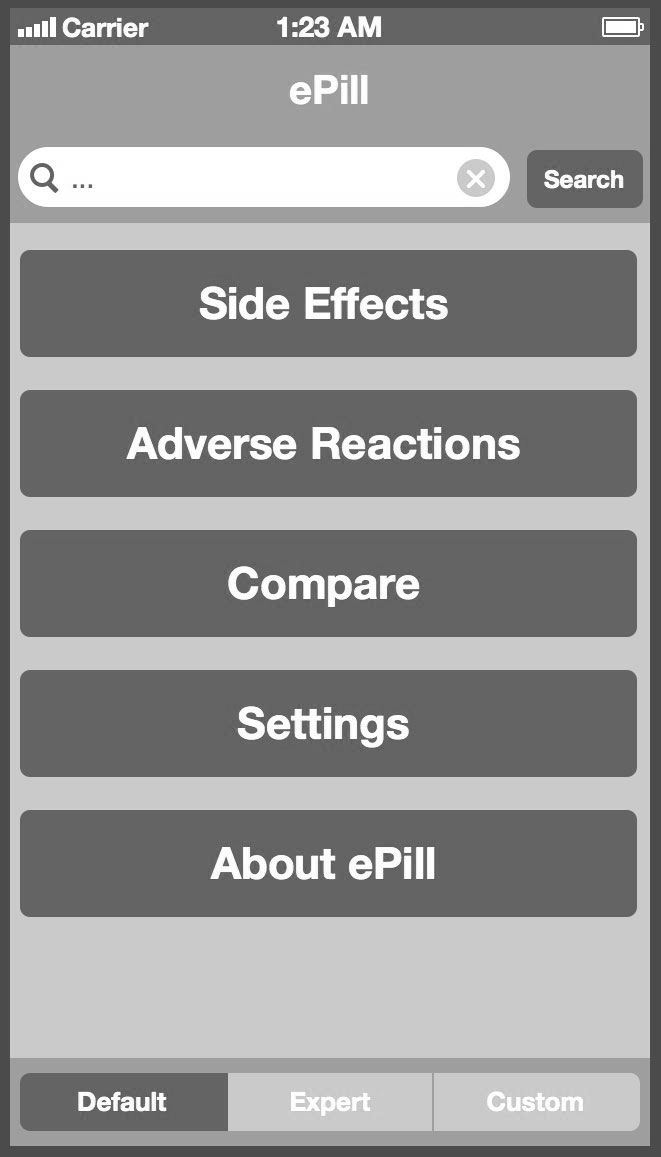
\includegraphics[width=0.8025\linewidth]{figures/Screen_1_bw.jpg}
        \caption[Main Screen Mockup]{Main Screen Mockup}
        \label{fig:Mockup}

    \end{minipage}
    \hspace{0.5cm}
    \begin{minipage}[b]{0.45\linewidth}
        \centering
        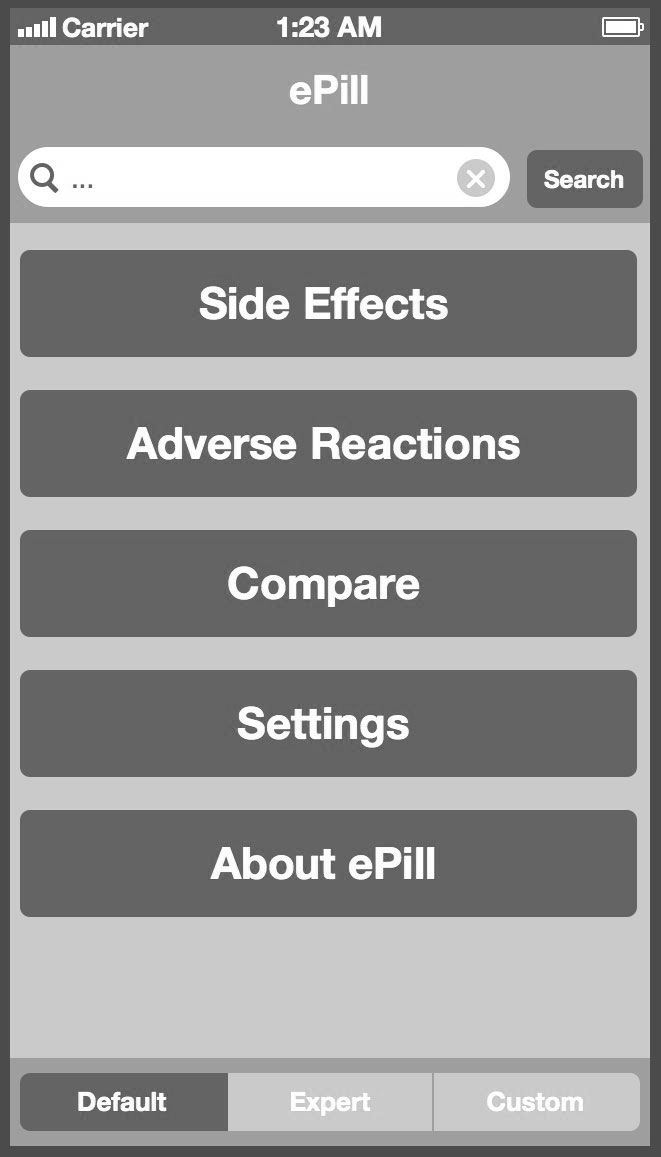
\includegraphics[width=0.8025\linewidth]{figures/Screen_1_bw.jpg}
        \caption[Final Main Screen]{Final Main Screen}
        \label{fig:FinalMainScreen}

    \end{minipage}
    \\
    \\
    \\
    \begin{minipage}[b]{0.45\linewidth}
        \centering
        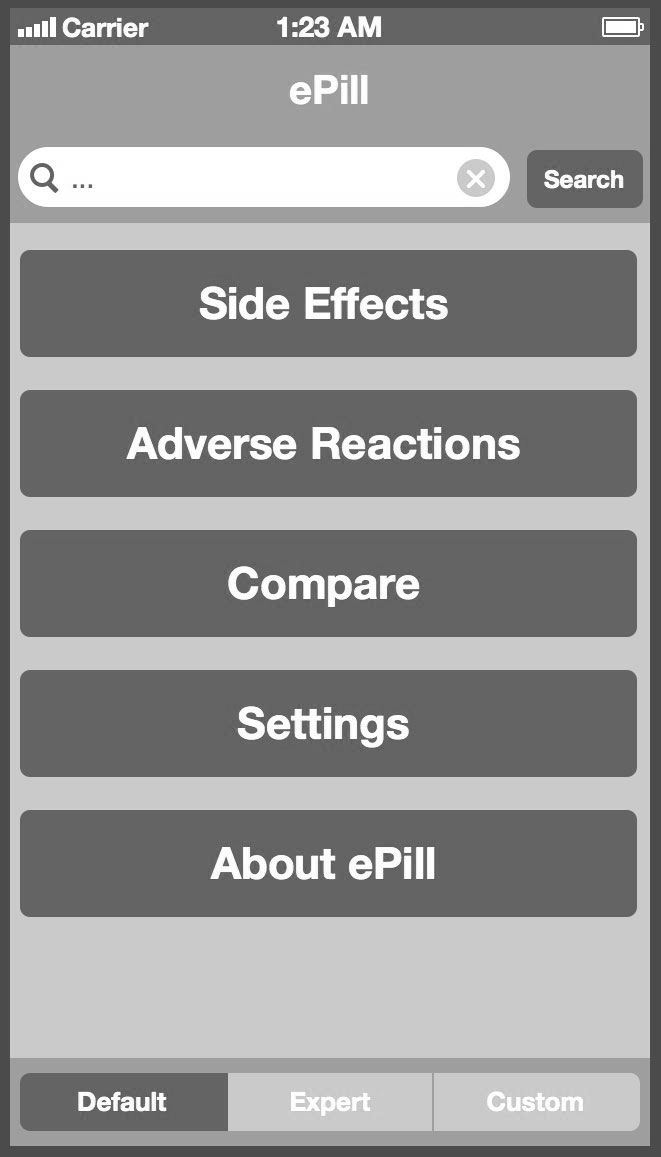
\includegraphics[width=0.8025\linewidth]{figures/Screen_1_bw.jpg}
        \caption[Search Input Screen]{Search Input Screen}
        \label{fig:SearchInputScreen}

    \end{minipage}
    \hspace{0.5cm}
    \begin{minipage}[b]{0.45\linewidth}
        \centering
        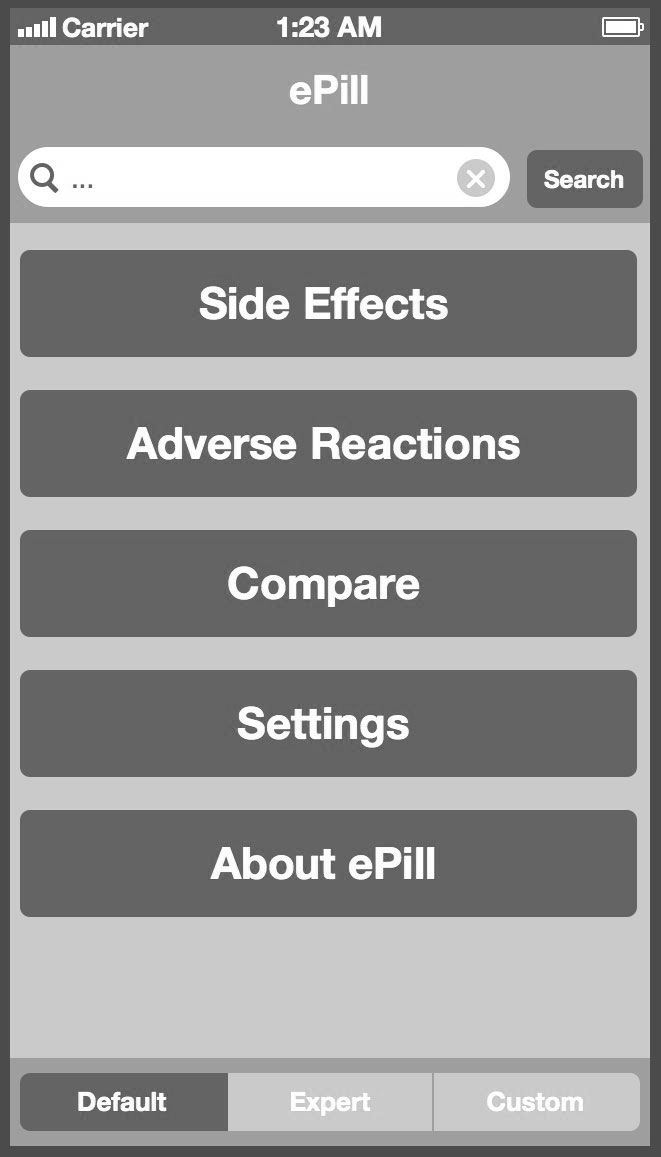
\includegraphics[width=0.8025\linewidth]{figures/Screen_1_bw.jpg}
        \caption[Search Result Screen]{Search Result Screen}
        \label{fig:SearchResultScreen}

    \end{minipage}
\end{figure}
\\
The three major functions of ePill (Search, Display and Supplementing Services) should be accessible as fast as possible. Of course, the display functionality and some supplementing services (e.g. the term explanation functionality) are only able to present results, if a pharmaceutical is selected. So we designed \ref{fig:Mockup} as a stripped down starting screen with every main function quickly available. Due to some missing generic controls provided by Vaadin TouchKit, like the search bar, we finally implemented the start screen as illustrated in \ref{fig:FinalMainScreen}. This resulted furthermore in a more separated presentation of search string input view and result view, as presented in \ref{fig:SearchInputScreen} and \ref{fig:SearchResultScreen}.
\\
\\
Throughout the planning and designing we tried to reproduce common patterns and user controls. Therefor we utilized the navigation back on the top left corner, illustrated by a leftwards oriented arrow-shaped button. Central navigation which specified the view, e.g. main function selection or the selection of a specific pharmaceutical from e.g. a search result list, is centered in the main content area in the screen's center.
\\
\\
Most of the views offer a toolbar at the screen's bottom. This toolbar contains controls which are used for navigation inside the screen's center view, e.g. go back to top or navigate to a specific header. Especially in the pharmaceutical details view with much information visible, it can be very handy to jump right to the header one is interested in. Additionally, some controls are added in the toolbar which enable further interaction with the information displayed, e.g. adding the currently visible pharmaceutical to the current list, which I will discuss later.
\\
\\
The web application has rich customization possibilities. One can adjust the font size, the details of pharmaceuticals to be displayed and the layout of the web application itself. As it turned out, it is not applicable for the user to change the mobile apps layout, because the user interface so too compact to add additional elements and too few elements are visible to hide any element.
\\
\\
The current list is a concept added to the mobile application and derived from a view in the web application. The web application offers a view in which pharmaceuticals can be added and afterwards, via a button click, aggregated information, like adverse reactions, can be listed. Because we have much less available screen space in the mobile app, we decided to have the list globally available throughout the entire app. E.g. if one searched for a pharmaceutical and has selected one to display detailed information, one can easily via a button in the toolbar add this pharmaceutical to one's current list. If one now selects e.g. the side effects functionality in the main screen, one sees his current list and can add more to it. This screen is illustrated in \ref{fig:CurrentListScreen}. If one decides to do so, one is presented a search input screen but can in the search result screen only tick on those pharmaceuticals one wants to add to one's current list and not see the pharmaceutical details on click. This is illustrated in \ref{fig:AlternativeListScreen}.
\begin{figure}[!tb]
    \begin{minipage}[b]{0.45\linewidth}
        \centering
        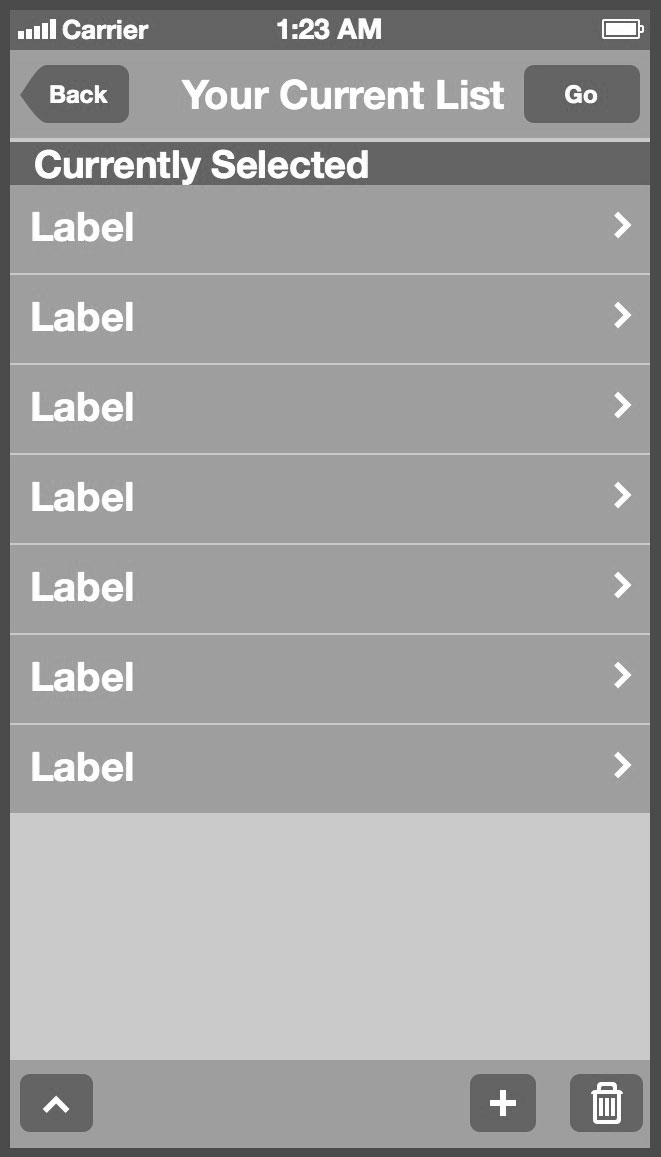
\includegraphics[width=0.8025\linewidth]{figures/Screen_2_bw.jpg}
        \caption[Current List Screen]{Current List Screen}
        \label{fig:CurrentListScreen}

    \end{minipage}
    \hspace{0.5cm}
    \begin{minipage}[b]{0.45\linewidth}
        \centering
        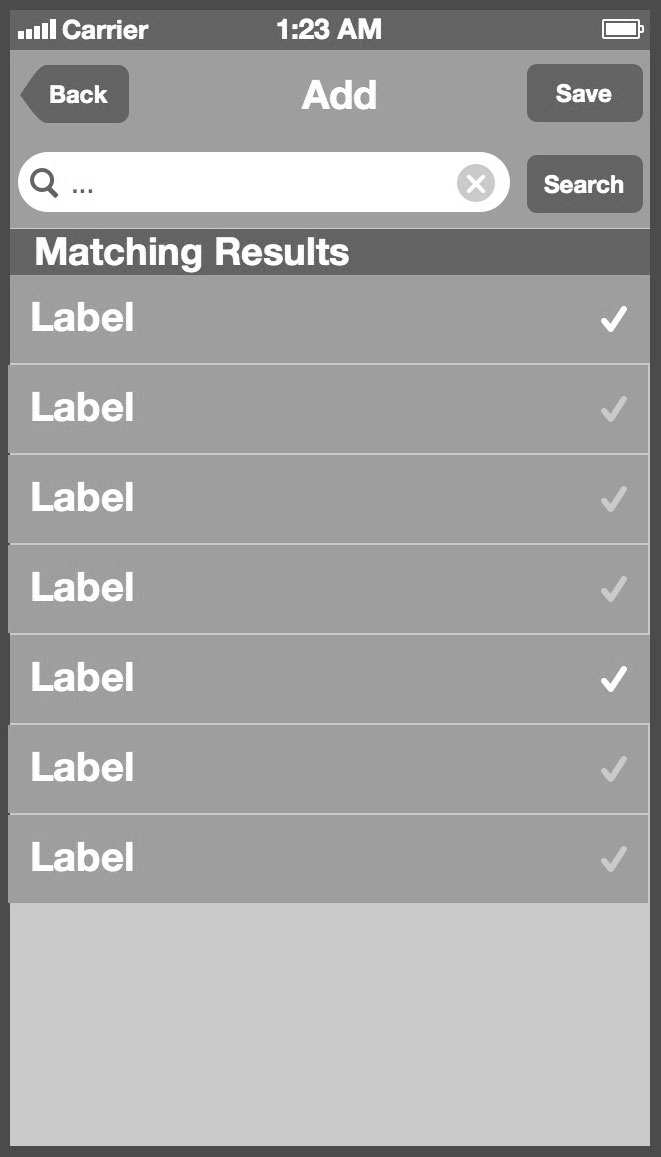
\includegraphics[width=0.8025\linewidth]{figures/Screen_3_bw.jpg}
        \caption[List Screen to add to Current List]{Alternative List Screen}
        \label{fig:AlternativeListScreen}

    \end{minipage}
\end{figure}

\subsection{The Implementation Process}
\label{subsec:Implementation}

\subsection{Validation of the mobile App}
\label{subsec:Validation}
\newpage
\section{Lessons Learned}
\label{sec:LessonsLearned}
mHealth apps do have some similar requirements as any app, but have to deal with much stronger information security concerns compared to casual apps. They also need to pay more attention to usability and availability than most other apps by definition.\footnote{cf \cite{WorldHealthOrganization.2011} cited by \cite{MartinezPerez.2013}, p. 2}
\\
In the case of ePill information security is not an issue because no user related information is stored. But developing with Vaadin was not always a good choice. Vaadin simplified the development process but slowed it down at the very beginning. The app is not as perfectly designed as it could have been with more influence on the final layout on the client-side, especially on the user interface in terms of available user interface controls.
\\
\\
After having read the Vaadins Beginner Guide\footnote{\url{https://vaadin.com/tutorial}, last visited on 09/21/2013} we only had minor issues understanding Vaadins architecture and development went mostly quick and easy. As already stated, some missing controls were a drawback to us and workarounds had to be found, but all in all it is a good solution for a quick development without the need of further knowledge in HTML, CSS or JavaScript. Having not to deal with cross-browser-optimizations was a relieve.
\\
After the development of the mobile app we would nevertheless propose a different approach. If Vaadin is already utilized in the existing system, it is good to reuse the code. But if not, or if a web service is available, we would suggest developing native applications, maybe with Xamarin\footnote{\url{http://xamarin.com}, last visited on 09/21/2013}. This offers the possibility to fine tune the user interface much more, offer a much more familiar look on the different OS and much more user interface controls are available. While the web app developed with Vaadin looks on all OS similar and similar to iOS, with native apps the different apps would incorporate themselves more into the environment of the OS. It is worth the additional effort of developing a standalone web service to provide the data for a mobile client and different user interfaces, at least their OS-specific definition for the better accessibility. Additionally, OS like iOS offer native apps the possibility to run in background and perform specific tasks energy efficiently, while web-based apps are forced to quit on exit. This constraint does not affect ePill but e.g. monitoring apps need a continuing execution.
\\
Frameworks such as PhoneGap\footnote{\url{http://phonegap.com}, last visited on 09/21/2013} provide accessibility to extended functionality of the device for most mobile OS but still do not offer background execution. For instance, Apple offers APIs only for native apps.\footnote{cf. \url{https://developer.apple.com/library/ios/documentation/iphone/conceptual/iphoneosprogrammingguide/ManagingYourApplicationsFlow/ManagingYourApplicationsFlow.html}, last visited on 09/24/2013} Android offers similar to Apple Services, the execution environment for long running tasks, only to native apps.\footnote{cf. \url{http://developer.android.com/guide/components/services.html}, last visited 09/24/2013}
\\
Using native apps also eases the integration of accessibility features such as font enlargement or voice guided navigation inside the app. Most modern OS provide many accessibility features which can not or only partially be utilized inside a web-based app. A voice-guided navigation could be useful for ePill for either impaired people or in situations in which one is not able to operate by touch.
\\
\\
We furthermore learned that planning plays an important role for a fast and successful implementation. For a successful planning, knowledge of the used software and their possibilities is important. During planning we had only superficial knowledge about Vaadin and TouchKit, we inspected sample code and user interfaces, which made us believe that most controls from native applications can be utilized as well. If we knew during development that many controls are not implemented already, our planned user interface would have looked different and we would have saved some time during the implementation.
\newpage
\section{Conclusion}

\newpage

% --------------------
% Literaturverzeichnis
% --------------------
\newpage
\patchcmd{\bibsetup}{\interlinepenalty=5000}{\interlinepenalty=10000}{}{}
\printbibliography[title={Bibliography}]
\addcontentsline{toc}{section}{Bibliography}


% ---------
% Anhang
% ---------
\section*{Erklärung}
\addcontentsline{toc}{section}{Erklärung}

Hiermit versichere ich an Eides Statt, dass ich die vorliegende Arbeit selbstständig und ohne die Benutzung anderer als der angegebenen Hilfsmittel angefertigt habe. 
Alle Stellen, die wörtlich oder sinngemäß aus veröffentlichten und nicht veröffentlichten Schriften entnommen wurden, sind als solche kenntlich gemacht. 
Die Arbeit ist in gleicher oder ähnlicher Form oder auszugsweise im Rahmen einer anderen Prüfung noch nicht vorgelegt worden.

\vspace{30mm}
\begin{flushleft}
    Köln, den 26. September 2013
\end{flushleft}
\section*{\hspace{0.2cm}Lebenslauf} 
\addcontentsline{toc}{section}{Lebenslauf}

\begin{flushleft}

% Persönliche Angaben
\begin{tabular}{p{11em} p{10em} p{10em}}
    \multirow{5}{*}{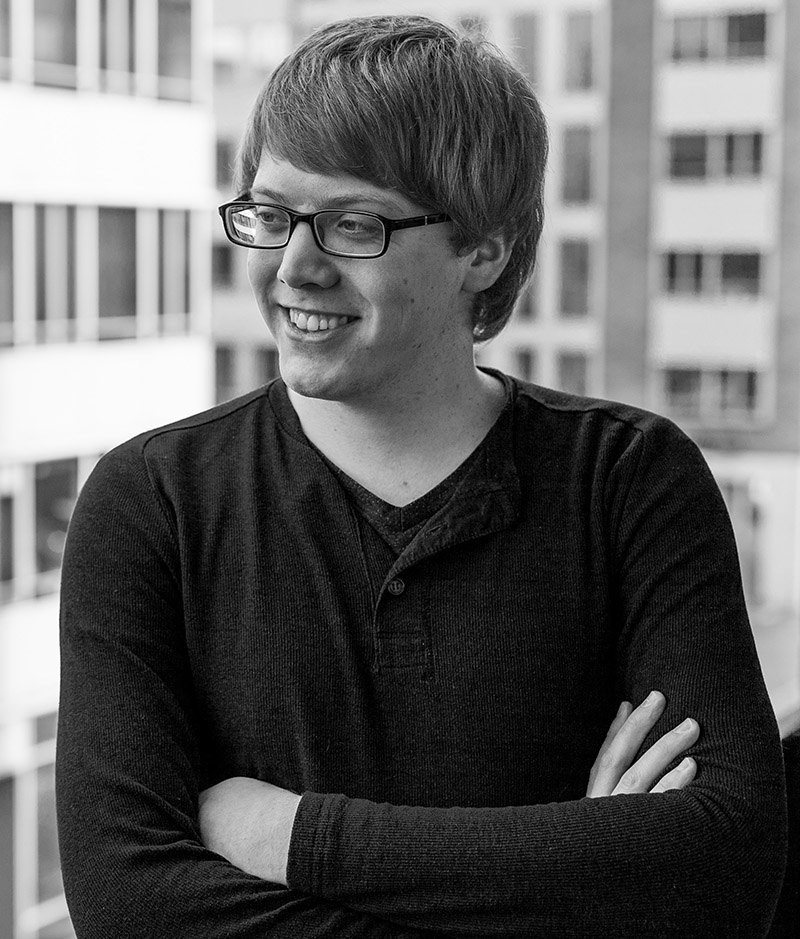
\includegraphics[width=40mm]{figures/passfoto.jpg}} & \textbf{Persönliche Angaben} & \addspace \\
    & Name: & Phil Diegmann \\
    & Anschrift: & Wipperfürther Str. 477, 51515 Kürten \\
    & Geburtsdatum und -ort: & 06.02.1991 in Wipperfürth \\
    & Familienstand: & ledig \\
\end{tabular}

\vspace{1.5em}

% Ausbildung
\begin{tabular}{p{11em} p{22.5em}}
    \textbf{Schulische Ausbildung} & \addspace \\
    1998 - 2002 & St. Antonius Grundschule in Wipperfürth \\
    2002 - 2010 & Engelbert-von-Berg Gymnasium in Wipperfürth, Abschluss: Abitur (1,5) \\
\end{tabular}

\vspace{0.5em}

% Studium
\begin{tabular}{p{11em} p{22.5em}}
    \textbf{Studium} & \addspace \\
    10/2010 - 09/2013 & Universität zu Köln, Wirtschaftsinformatik, Bachelor of Science \\
    10/2013 - 09/2015 & Universität zu Köln, Information Systems, Master of Science
\end{tabular}


\vspace{-1em}

% Praktika

% Beruflicher Werdegang

\end{flushleft}

\end{document}